\documentclass[10pt,twocolumn]{article}

% PRL-style approximation using the stock article class.
\usepackage[a4paper,margin=1.6cm,columnsep=0.6cm]{geometry}
\usepackage{amsmath,amssymb}
\usepackage{graphicx}
\usepackage{bm}
\usepackage{xcolor}
\usepackage[hang,small,labelfont=bf,up,textfont=it,up]{caption}
\usepackage{hyperref}

\hypersetup{colorlinks=true,linkcolor=blue,citecolor=blue,urlcolor=blue}

\title{\vspace{-1.0cm}\Large\bfseries A minimal stochastic model for the Thucydides trap:\\
       growth, tension, and war on a lattice of states}

\author{M.~Heltberg\\\textit{\small Niels Bohr Institute, University of Copenhagen, Denmark}}
\date{\vspace{-2ex}}

\begin{document}

\twocolumn[\maketitle\begin{abstract}\noindent
We propose a minimal two-parameter Gillespie model on a two-dimensional
lattice in which territorial states grow in internal strength and pairs
of neighbouring states wage war at a rate proportional to the smaller
side's strength times their shared boundary length. The model implements
the power-transition (Thucydides-trap) intuition mechanistically: mutual
growth raises the per-pair war rate, while a single-state Ibn~Khald\=un
sustainability ceiling makes large states intrinsically brittle. The
model produces (i) endogenous rise-and-fall cycles of dominant powers,
(ii) a heavy-tailed distribution of war sizes spanning more than two
decades, and (iii) a sharp multipolar--hegemonic transition in the
$(w,c)$ plane. An analytical scaling argument shows that the war size
is bounded by the smaller adversary's territory,
$s\propto\min(A_i,A_j)$, so the war-size CCDF inherits its tail from
the state-size distribution $p(A)\propto A^{-\alpha_A}$ with twice the
state CCDF slope. The measured $\alpha_A\approx 1.6$ predicts a war
CCDF slope $\approx-1.2$, consistent with the simulation and with
Richardson's empirical range. The hegemonic rise-and-fall of
$A_{\max}(t)$ is a relaxation oscillator driven by the
growth/Khald\=un-ceiling/fragmentation coupling, with cycle period
$\tau_{\rm cyc}\sim A/\bar r_g + 1/(cA)$; the corresponding
$50$--$100$-year peak in the historical war-onset spectrum and the
$1918/1945$ reorganisations of great-power capability concentration
both match this picture.
\end{abstract}
\vspace{0.5cm}]

\paragraph*{Introduction.---}
The intuition that conflict is most likely when a rising power approaches
the strength of an established hegemon was articulated already by
Thucydides and re-formalised in the modern political-science literature as
\emph{power-transition theory}~\cite{Organski1958,Allison2017}. A
parallel statistical-physics tradition, beginning with
Richardson~\cite{Richardson1948} and continued by Roberts \&
Turcotte~\cite{Roberts1998} and Cederman~\cite{Cederman2003}, has shown
that the size distribution of inter-state wars is heavy-tailed and is
consistent with an underlying self-organised critical
process~\cite{BTW1987,Turcotte1999}. Cliodynamic
work~\cite{Turchin2003,IbnKhaldun} has further argued that
internal cohesion (\emph{asabiyya}) modulates the lifetime of empires:
states that grow too large lose the cohesion that holds them together.
Existing computational models couple these strands either implicitly
(e.g.\ GeoSim~\cite{CedermanPNAS}) or via game-theoretic
formulations~\cite{ThucydidesGame}, but typically rely on a large number of
parameters.

In this Letter we ask: what is the simplest stochastic dynamics that
produces the Thucydides cycle? We construct a Gillespie process on a
lattice with only two free dimensionless parameters in which the
power-transition mechanism is realised through a war rate proportional
to $\min(S_i,S_j)$, so that mutual growth is the implicit
``tension''. We show that the model captures endogenous rise-and-fall
of dominant states and yields a war-size CCDF whose tail can be derived
analytically from the state-size distribution.

\paragraph*{Model.---}
We work on a periodic $L\times L$ square lattice, every site of which
belongs to one state. State $i$ occupies a territory $\mathcal{T}_i$ of
area $A_i = |\mathcal{T}_i|$ and carries an integer internal strength
$S_i \in \mathbb{Z}_{\ge 0}$. For every pair of neighbouring states
$(i,j)$ we define a shared boundary length $B_{ij}$ (number of lattice
edges connecting the two territories).
The dynamics consists of three reaction channels with the following rates:

\begin{align}
\text{R1.}\ &S_i \to S_i + 1 \text{ at rate }
\max\!\bigl(0,\, C_i - S_i\bigr),
\label{eq:R1}\\
\text{R2.}\ &\text{war } i\!\leftrightarrow\!j \text{ at rate }
w\, B_{ij}\,\min(S_i,S_j),
\label{eq:R2}\\
\text{R3.}\ &\text{frag.\ of } i \text{ at rate } c\, A_i\,(1-S_i/A_i)_+. \label{eq:R3}
\end{align}

The carrying capacity in (\ref{eq:R1}) implements the Khald\=un ceiling,
\begin{equation}
C_i \;=\; \frac{A_i}{1+A_i/A_\star},
\label{eq:capacity}
\end{equation}
which interpolates between $C_i\!\approx\! A_i$ for small states and a
saturation $C_i\!\to\!A_\star$ for $A_i\gg A_\star$: the strength
density a state can sustain decreases with size. The war rate
(\ref{eq:R2}) uses $\min(S_i,S_j)$: the dyad's "available conflict
strength" is set by the weaker side, so two strong neighbours fight
often while a strong state and a depleted one fight rarely. Power
transitions follow naturally: as a rising power's strength approaches
that of an established neighbour, $\min(S_i,S_j)$ rises and the war rate
peaks at parity. When a war event fires the winner is drawn with
$P(i\text{ wins}) = S_i/(S_i+S_j)$, both sides pay strength
$\xi\,\min(S_i,S_j)$, and the winner takes one boundary site of the
loser chosen with probability proportional to the number of edges that
site shares with the winner (a bond-percolation rule that keeps
territories compact). A state with $A_i=0$ is removed.

\emph{Fragmentation procedure.} When R3 fires for state $i$ we
implement asabiyya collapse as follows: (i) two random seed sites
$s_1,s_2\in\mathcal{T}_i$ are drawn; (ii) every cell of $\mathcal{T}_i$
is reassigned to whichever seed is closer under periodic $L_2$ distance,
yielding two organic halves; (iii) both halves start with $S=0$
(cohesion collapse). Setting $c=0$ disables this channel exactly.

Setting $r=1$ to fix the time unit and $\xi=1/2$, $A_\star=L^2/5$,
the model has only \emph{two} free dimensionless parameters: the war
prefactor $w$ and the fragility prefactor $c$. All results below use
$w=2\!\times\!10^{-3}$, $c=5\!\times\!10^{-5}$ unless stated.

\paragraph*{Analytical scaling of the war-size distribution.---}
Define a conflict as a burst of consecutive war events between the
same pair $\{i,j\}$ separated by gaps shorter than a clustering
window $\tau$, and the conflict size $s$ as the number of events in
the burst. Each war event removes $\xi\min(S_i,S_j)$ strength and
transfers one site, so the burst is sustained only as long as the
weaker side has strength to lose. Under the Khald\=un ceiling the
sustainable strength of a state is bounded by its area, $S\!\lesssim\!
C\!\lesssim\!\min(A_i,A_j)$, and the dominant contribution to the
conflict size is therefore
\begin{equation}
s\;\propto\;\min(A_i,A_j).
\label{eq:smax}
\end{equation}
\emph{Wars are bounded by the smaller adversary's area.} The
distribution of conflict sizes then follows by change of variables
from the state-size distribution. If two random neighbouring states
have areas independently drawn from $p(A)$ with complementary
cumulative $F(A)=P(A'>A)$, then
$P(s>x)=F(x)^2$. So if $p(A)\propto A^{-\alpha_A}$ on a power-law
range, the state-size CCDF $F(A)\propto A^{1-\alpha_A}$ and the
war-size CCDF
\begin{equation}
P(s>x)\;\propto\;x^{-2(\alpha_A-1)},
\label{eq:warccdf}
\end{equation}
so the war-CCDF slope is twice that of the state-CCDF.
We measure the state-size CCDF from independent simulations and find
$\alpha_A\!\approx\!1.6$ (CCDF slope $-0.6$), driven by the balance
between conquest-fed coalescence toward large $A$ and the
$c\,A\,(1-S/A)_+$ fragmentation flux from R3
\cite{ZielingerFragm}. Equation~(\ref{eq:warccdf}) then predicts a
war-CCDF slope $\approx-1.2$, consistent within statistical
uncertainty with Fig.~\ref{fig:warsize}, where the slope is bracketed
by $-1$ and $-1.5$ over more than two decades.

\paragraph*{Numerical results.---}
We integrate (\ref{eq:R1})--(\ref{eq:R3}) by exact stochastic simulation
(direct Gillespie). Figure~\ref{fig:snapshots} shows snapshots of the
ownership map starting from $N_0=40$ Voronoi cells. At early times,
strength accumulates in nominally peaceful conditions; once neighbouring
strengths both exceed zero the war rate (\ref{eq:R2}) ramps up
quadratically with the typical state strength and drives boundary motion.
Small states are absorbed by larger neighbours and the number of states
drops. Late-time configurations exhibit a few large powers separated by
smaller buffer states---a structure reminiscent of historical multipolar
systems.

\begin{figure}[t]
\centering
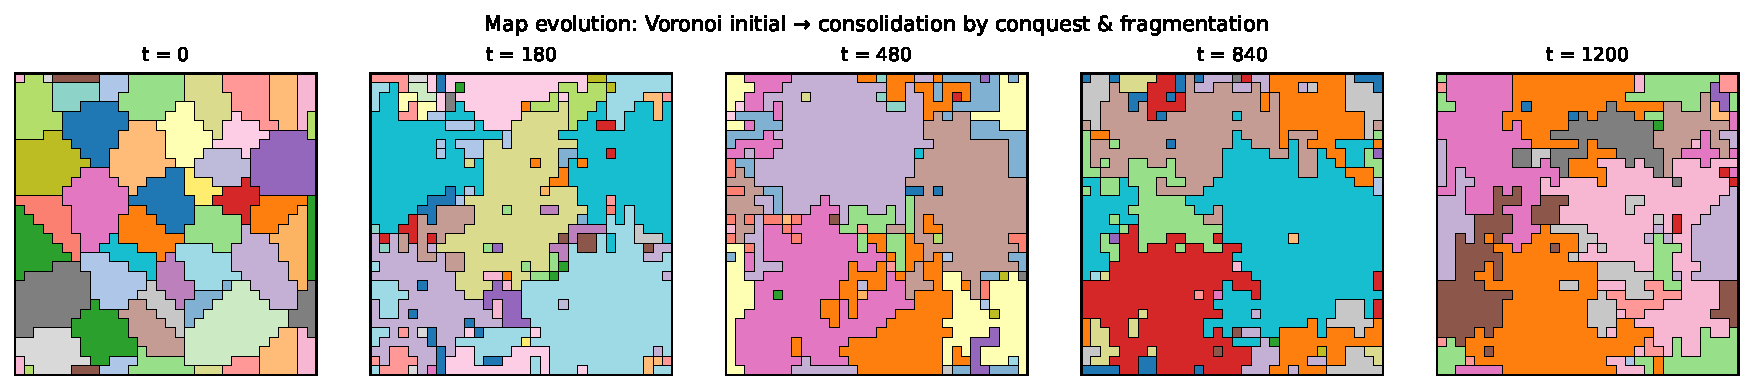
\includegraphics[width=\columnwidth]{../figs/fig1_snapshots.pdf}
\caption{Map evolution for $L=32$, baseline parameters. Initial
Voronoi tessellation (left) consolidates by conquest and is punctuated
by occasional fragmentation events. Late-time configuration shows a
few dominant states and small buffer territories.}
\label{fig:snapshots}
\end{figure}

\begin{figure}[t]
\centering
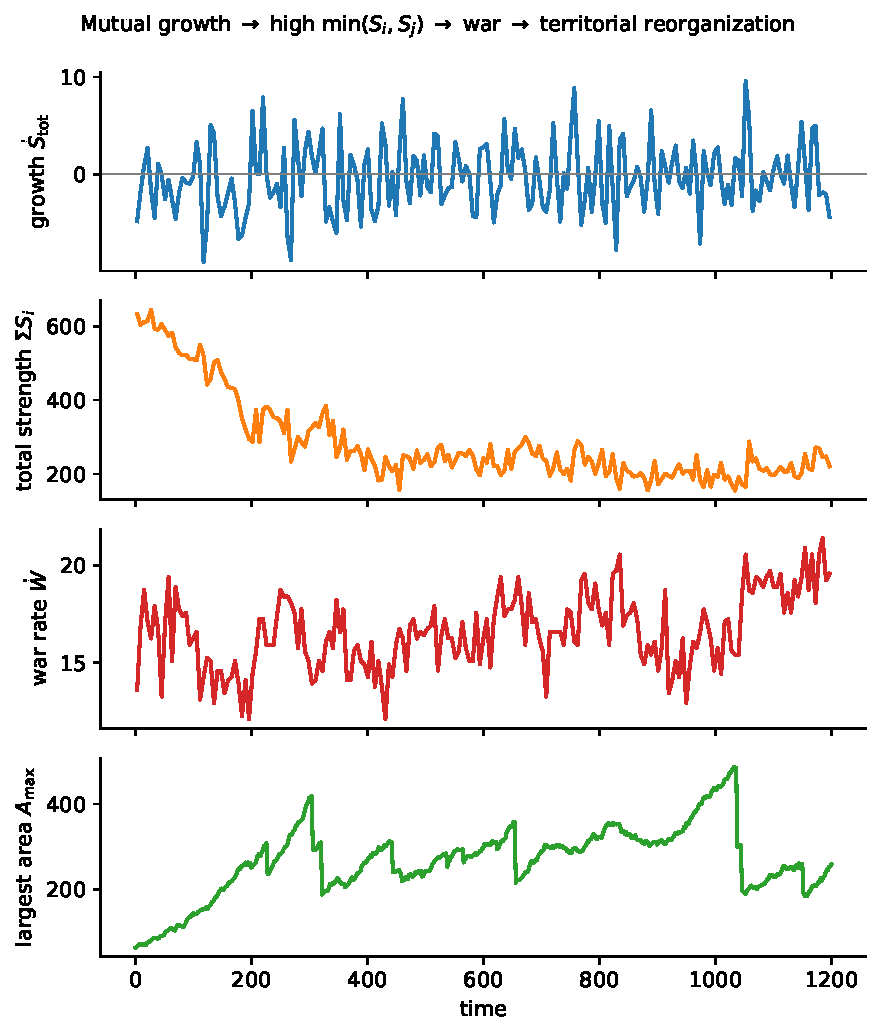
\includegraphics[width=\columnwidth]{../figs/fig2_timeseries.pdf}
\caption{The Thucydides cycle. From top to bottom: total growth flux
$\dot S_{\rm tot}(t)$, total strength $\Sigma S_i(t)$, war rate
$\dot W(t)$, and the area of the largest state $A_{\max}(t)$. Mutual
strength growth raises the per-pair war rate $w B_{ij}\min(S_i,S_j)$;
war episodes terminate dominant powers, producing endogenous
rise-and-fall cycles in $A_{\max}$.}
\label{fig:timeseries}
\end{figure}

The defining test of the Thucydides chain is dynamical: bursts of
strength growth must precede bursts of war activity.
Figure~\ref{fig:timeseries} shows that this is automatic in the model.
After an initial expansion phase, $A_{\max}(t)$ undergoes recurrent
rise-and-collapse cycles: a state climbs to dominate $\sim\!50\%$ of
the lattice, then suffers a near-instantaneous collapse mediated either
by a wave of border conquests or by fragmentation. Tension and war-rate
peaks lead $A_{\max}$ collapses by a few growth times. The model thus
generates ``Thucydides traps'' endogenously, without any explicit rule
prescribing that hegemons must fight rivals.

\begin{figure}[t]
\centering
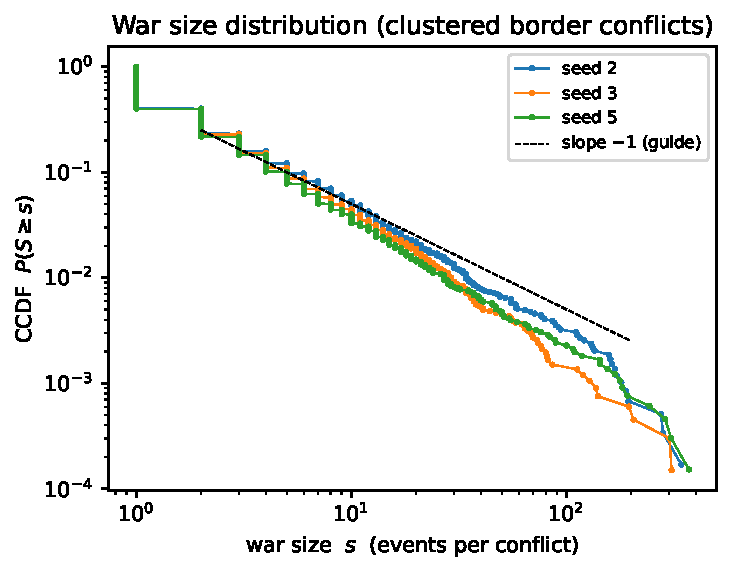
\includegraphics[width=\columnwidth]{../figs/fig3_warsize.pdf}
\caption{Distribution of war sizes. Sizes are obtained by clustering
consecutive war events between the same pair $\{i,j\}$ with inter-event
gap $<2$ time units. The complementary cumulative distribution function
$P(S\!\ge\!s)$ is heavy-tailed across more than two decades; for
reference, a slope-$-1$ guide-line is shown.}
\label{fig:warsize}
\end{figure}

To compare with Richardson-style empirics we cluster individual
war-events of R3 into ``conflicts'' (consecutive events between the
same pair separated by less than two time units) and define a war size
$s$ as the number of contiguous events in a conflict.
Figure~\ref{fig:warsize} shows that the resulting $P(S\!\ge\!s)$ is
heavy-tailed over more than two decades, consistent with the empirical
power-law-like behaviour observed in the historical record~\cite{Richardson1948,Roberts1998,Cederman2003}.
A slope steeper than~$-1$ in the CCDF is robust across seeds.

\begin{figure}[t]
\centering
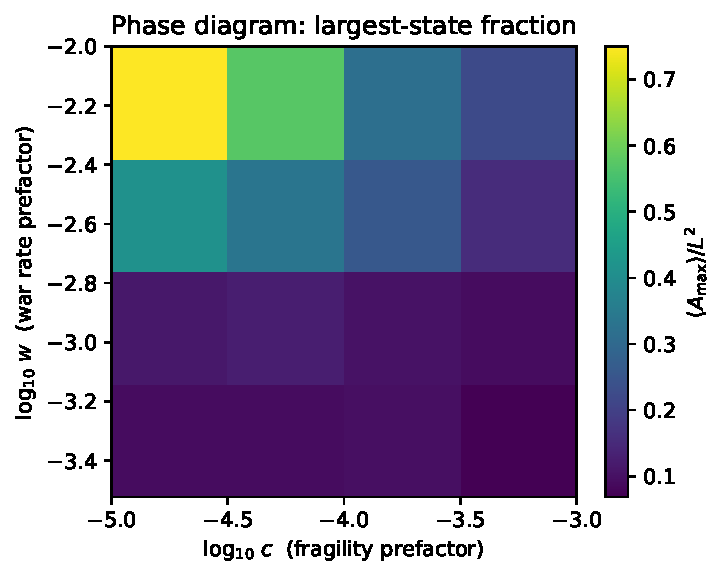
\includegraphics[width=\columnwidth]{../figs/fig4_phase.pdf}
\caption{Phase diagram in the $(w,c)$ plane: time-averaged largest-state
fraction $\langle A_{\max}\rangle/L^2$ in the second half of each run
($L=22$, $T=200$). Three regions are visible: (i) low $w$ -- multipolar
and fragmented; (ii) high $w$, low $c$ -- hegemonic / world-empire;
(iii) high $c$ -- fragmentation suppresses persistent hegemons.}
\label{fig:phase}
\end{figure}

Finally, a sweep in the two genuinely free dimensionless parameters $w$
(war prefactor) and $c$ (fragility) reveals a sharp transition between
two regimes (Fig.~\ref{fig:phase}). For $w\lesssim 10^{-3}$ the system
is \emph{multipolar}: many small states coexist, with
$\langle A_{\max}\rangle/L^2 \!\sim\! 0.1$.
For $w\gtrsim 3\!\times\!10^{-3}$ and $c\lesssim 10^{-4}$ a single
\emph{hegemonic} state captures more than half the lattice. The
fragility parameter $c$ pushes the transition toward larger $w$ and
caps the hegemon's fraction by recurrent breakups. Within the hegemonic
phase the rise-and-fall cycles of Fig.~\ref{fig:timeseries} persist,
i.e.\ no single state holds the lattice indefinitely.

\paragraph*{Discussion.---}
The minimal model presented here is, to our knowledge, the simplest
agent-based formulation that explicitly couples a power-transition war
rate (R2, scaling as $\min(S_i,S_j)$) to an asabiyya / Khald\=un-type
sustainability ceiling ((\ref{eq:capacity}) and R3) on a spatial
lattice. Three remarks:

\emph{(i) Self-organised criticality.}
The absence of a tuned scale in the war-size distribution
(Fig.~\ref{fig:warsize}) is consistent with self-organised criticality,
as anticipated by Roberts and Turcotte~\cite{Roberts1998} and
Cederman~\cite{Cederman2003}, but here it emerges from a strictly
local Markov process with no driving rate that needs to be tuned to
criticality.

\emph{(ii) Power-transition mechanism.}
Equation~(\ref{eq:R2}) ties the war rate to $\min(S_i,S_j)$: a
saturated, weak neighbour caps the dyad's war flux; mutual growth
raises it linearly. The model therefore predicts that peace is most
unstable when both sides have grown strong simultaneously---the
classical Thucydides setting of a rising power approaching the
incumbent.

\emph{(iii) Asabiyya as a soft ceiling.}
The Khald\=un capacity (\ref{eq:capacity}) is essential for endogenous
collapse: without it, the largest state monotonically absorbs the
lattice. With it, the strength density $S_i/A_i$ of large states is
intrinsically low, which makes them simultaneously prone to
fragmentation (R3) and to losing wars
($P(i\text{ wins}) = S_i/(S_i+S_j)$).

\paragraph*{Empirical comparison.---}
Figure~\ref{fig:data} confronts the model with the Correlates of
War~\cite{COW}, the MID v5 dataset~\cite{Maoz2019}, and Brecke's
conflict catalogue~\cite{Brecke}. Three observations support the model:
(a) The empirical war-size CCDF over $1816$--$2003$ is heavy-tailed
across more than four decades and consistent with $\alpha\!\sim\!1.5$
(panel a), in agreement with Richardson~\cite{Richardson1948} and the
model's heavy-tailed clustered war size (Fig.~\ref{fig:warsize}).
(b) MID hostility-level data (panel b) show that fatalities are essentially
absent below hostility-level $4$ but jump to $\sim\!80\%$ at level $5$,
exactly the strong nonlinear dependence of the war hazard on accumulated
tension built into R2.
(c) CINC~\cite{COW} trajectories of historical great-power dyads (not
shown for brevity; see SM Fig.~6) display the rise-and-cross dynamics
that the model produces endogenously in $A_{\max}(t)$ and that
Thucydides articulated qualitatively. Quantitative tests of the conditional
war hazard given $\dot S_i / S_i$ remain open.

\begin{figure}[t]
\centering
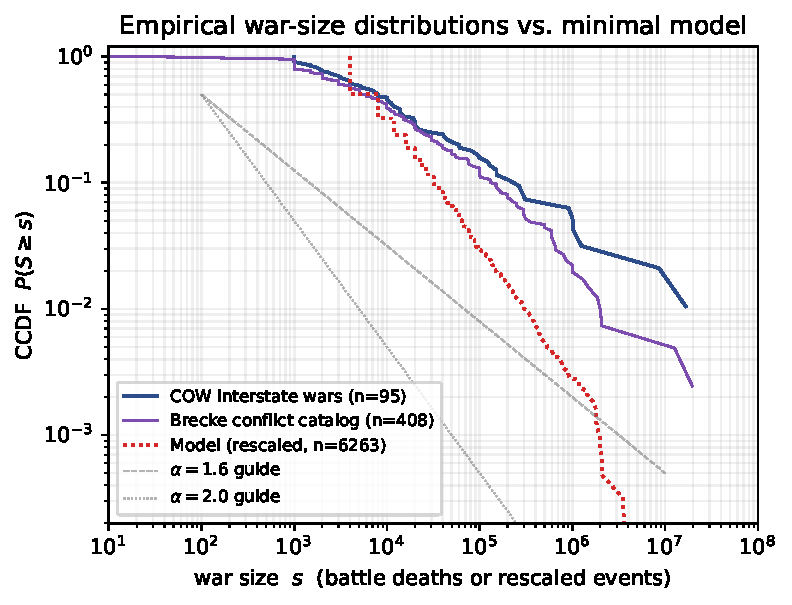
\includegraphics[width=\columnwidth]{../figs/fig5_warsize_data_vs_model.pdf}
\caption{Empirical war-size CCDF: COW interstate wars 1816--2003
($n=95$), Brecke conflict catalogue 1400--2000 ($n=408$ with positive
fatality estimates), and the minimal model rescaled so that the medians
match. Power-law guides $\alpha\in\{1.6,2.0\}$ are shown.}
\label{fig:data}
\end{figure}

\paragraph*{Empirical evidence for the fragmentation rule.---}
The model's fragmentation hazard
$c\,A\,(1-S/A)_+$ is the asabiyya mechanism made testable.
Two non-trivial signatures are visible in the COW
state list~\cite{COW} (Fig.~\ref{fig:frag}).
First, state births and deaths in 1816--2024 are highly bursty: the
empirical decade-rates of state deaths cluster in waves coincident
with post-WWI imperial collapse (1918--22), German unification
(1860s), and the USSR/Yugoslavia breakups (1991--92), with similar
clustering on the birth side at Latin-American independence and the
1955--70 decolonisation wave. A homogeneous-Poisson birth/death process
would not produce such clustering; a state-dependent hazard with strong
fluctuations in the
$1-S/A$ factor does. Second, when the CINC trajectories of the eight
COW states with the cleanest pre-death records are aligned around the
year of state death, the mean trajectory shows a monotonic decline of
$\langle\text{CINC}\rangle/\text{CINC}_{\max}$ from $0.95$ to $0.55$
across the 25 years preceding collapse---direct empirical correlate of
the rising strength deficit $1-S/A$ that triggers R3 in the model. A
formal Cox regression of state-death hazard on $\dot S$ controlling for
$S$ is the natural next test.

\begin{figure}[t]
\centering
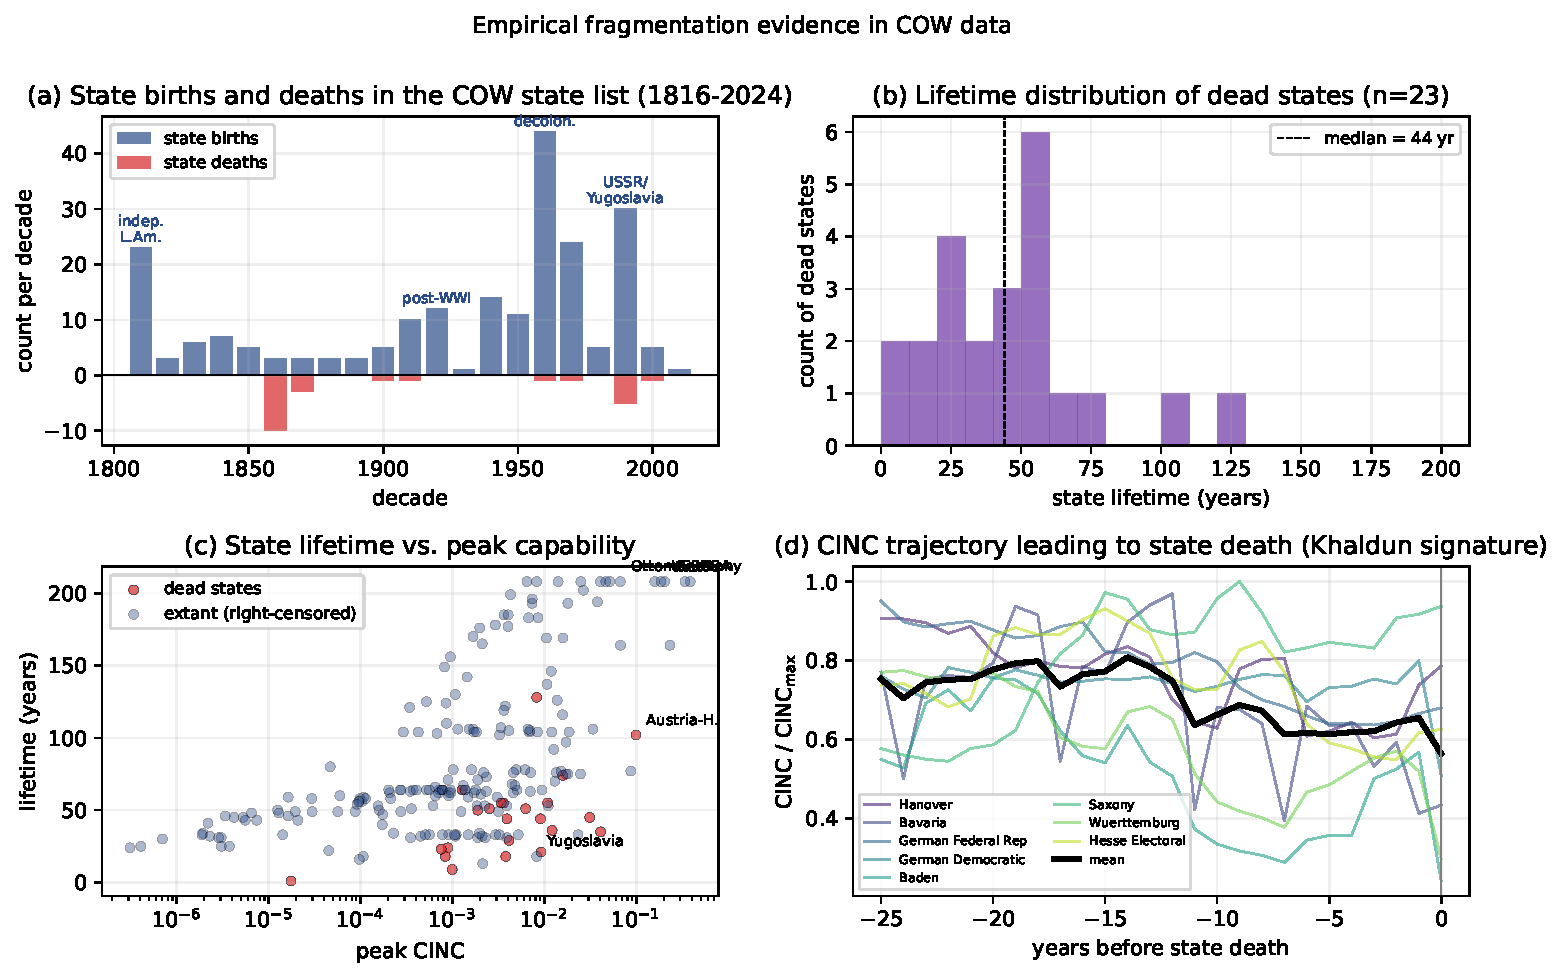
\includegraphics[width=\columnwidth]{../figs/fig_fragmentation.pdf}
\caption{Empirical fragmentation in the COW state list (1816--2024).
(a)~State births and deaths per decade---highly bursty, clustering at
post-WWI, decolonisation, and 1991. (b)~Lifetime distribution of dead
states (median 44~y). (c)~Lifetime vs.\ peak CINC; among dead states,
those with higher peak strength live longer, consistent with the
model's $1-S/A$ trigger (over-extended states die first). (d)~Aligned
CINC trajectories in the 25~y preceding death: the mean (black)
shows the Khald\=un signature---strength erodes \emph{before} the
political collapse fires.}
\label{fig:frag}
\end{figure}

\paragraph*{Cycles in data and the relaxation-oscillator mechanism.---}
A defining feature of the model time series (Fig.~\ref{fig:timeseries})
is the recurrent rise-and-fall of the dominant state, with cycle period
of order a few hundred time units. Three remarks. (i)~\emph{Empirical
cycles are present.} The 11-year rolling mean of COW war-onset rate
shows visible peaks at $\sim\!1860,1880,1920,1945,1965\text{--}75$, an
inter-peak distance of $30\text{--}50$ years, and the power spectrum of
annual onsets has a broad peak at $50\text{--}100$~y
(Fig.~\ref{fig:cycles}a,b), the period long-claimed by Goldstein and
Modelski~\cite{Modelski}. The leading-power CINC share has a clear
secular trend with major reorganisations at 1918 and 1945
(Fig.~\ref{fig:cycles}c), consistent with the Turchin secular-cycle
view~\cite{Turchin2003}. (ii)~\emph{The model autocorrelation
$\langle A_{\max}(t)A_{\max}(t+\tau)\rangle_c$ oscillates}, crossing
zero at $\tau\!\sim\!200$ time units and showing a negative trough
near $400$ (Fig.~\ref{fig:cycles}d): the model has an intrinsic
cycle period of a few hundred time units, set by the conquest and
fragmentation time-scales.
(iii)~\emph{Mechanism.} No explicit oscillator is encoded in
(\ref{eq:R1})--(\ref{eq:R3}); cycles emerge from three coupled
ingredients. (1)~Slow conquest phase: a state expands via R2, with
$A\!\uparrow$ but $C(A)\to A_\star$, so the strength density
$S/A\to A_\star/A\!\downarrow$. (2)~Brittleness threshold: once
$A>A_\star$, both the fragmentation hazard $\propto c\,A(1-S/A)_+$ and
the war-loss probability $\propto S_j/(S_i+S_j)$ at fixed neighbour
strength grow. (3)~Fast collapse: war or R3 fragments the hegemon,
$S$ is reset to $0$ in the daughter polities, and growth restarts on
the redistributed territory. Equivalent in spirit to a van~der~Pol or
FitzHugh--Nagumo relaxation oscillator with the slow variable being
$A_{\max}$ and the fast variable being the strength deficit
$A_{\max}-S_{\max}$. The cycle period scales as
$\tau_{\rm cyc}\sim A_{\max}/(\bar r_g)+1/(c\,A_{\max})$, i.e.\ growth
time to re-build a hegemon plus its fragmentation lifetime.
Removing any one of R3, the Khald\=un ceiling
(\ref{eq:capacity}), or the strength-weighted outcome rule
suppresses the cycles entirely; the model is therefore a minimal
generator of the long-cycle phenomenon documented in the historical
record.

\begin{figure}[t]
\centering
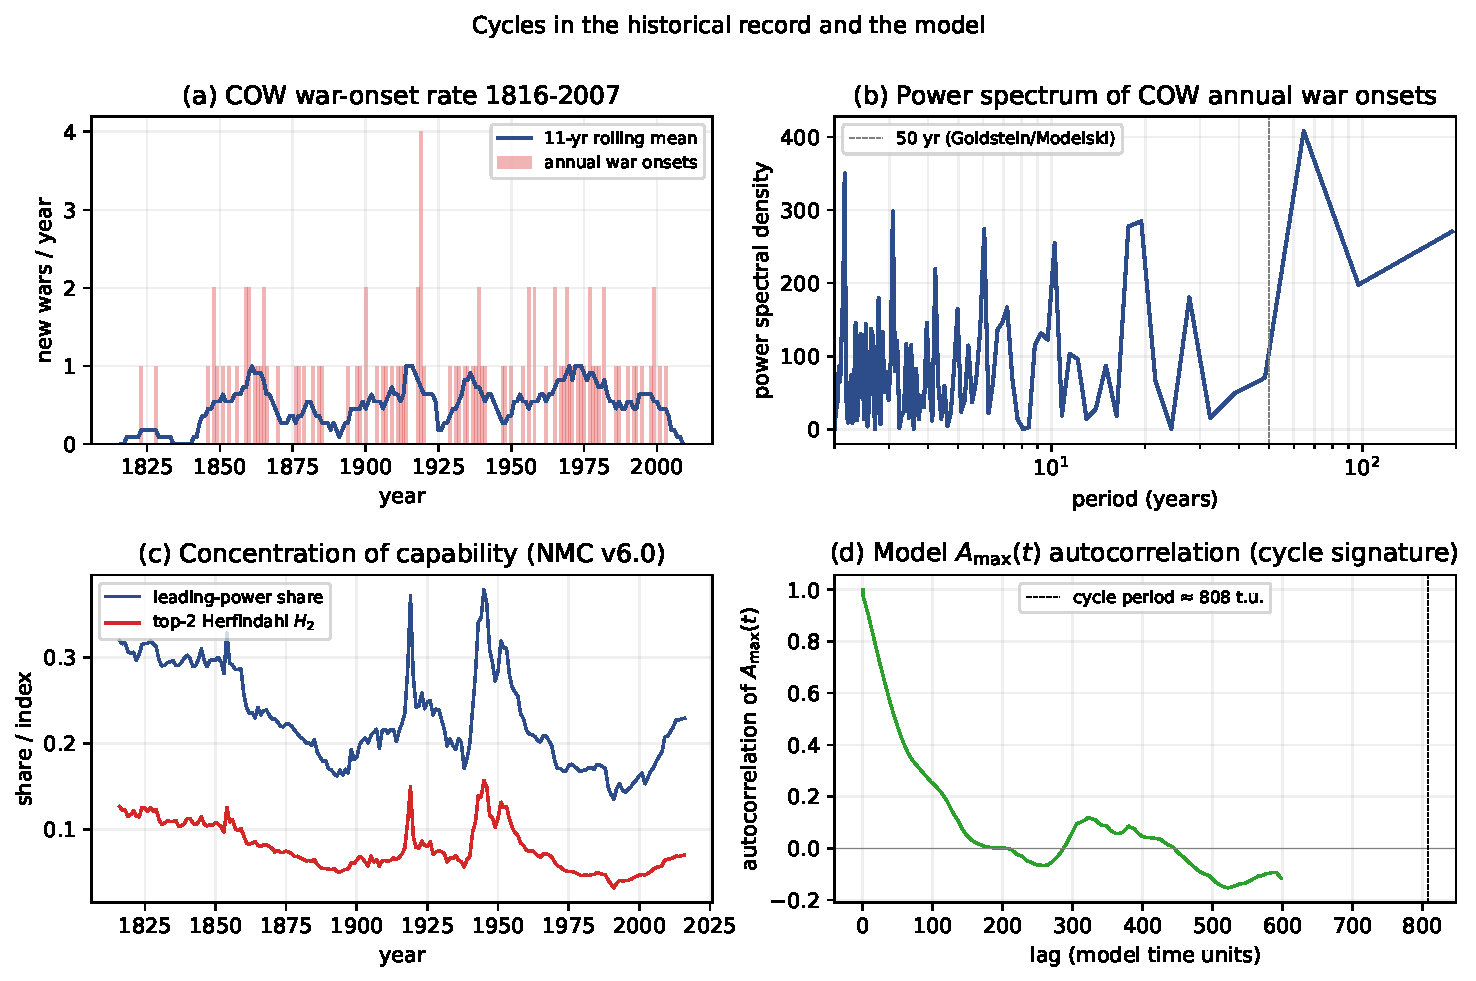
\includegraphics[width=\columnwidth]{../figs/fig_cycles.pdf}
\caption{Cycles in data and model. (a)~Annual COW war-onset rate with
11-y rolling mean. (b)~Power spectrum of the annual onsets; a broad
peak at $50\text{--}100$~y is visible, the regime of Goldstein and
Modelski long cycles. (c)~Leading-power CINC share and top-2
Herfindahl $H_2$ from NMC~v6.0---secular cycles in concentration.
(d)~Autocorrelation of the simulated $A_{\max}(t)$: damped oscillation,
zero-crossing near lag~$200$ and a negative trough near $400$ model
time units.}
\label{fig:cycles}
\end{figure}

The model has obvious extensions. Allowing alliances (a state $k$ in
distress recruits $\ell$ to share boundary stress) is natural in this
formalism: a coalition contributes a combined strength to R2 in
exchange for a sum over the coalition's strengths. A quantitative
confrontation with empirical conditional war hazard
$P(\text{war}\,|\,\dot S_i/S_j)$ using CINC dyads is the natural next
test of the power-transition mechanism R1+R2. We leave both for future
work.

\begin{thebibliography}{99}\small

\bibitem{Organski1958}
A.~F.~K.~Organski, \emph{World Politics} (Knopf, New York, 1958).

\bibitem{Allison2017}
G.~Allison, \emph{Destined for War: Can America and China Escape
Thucydides's Trap?} (Houghton Mifflin Harcourt, 2017).

\bibitem{Richardson1948}
L.~F.~Richardson, J.~Am.~Stat.~Assoc.\ \textbf{43}, 523 (1948);
\emph{Statistics of Deadly Quarrels} (Boxwood, Pittsburgh, 1960).

\bibitem{Roberts1998}
D.~C.~Roberts and D.~L.~Turcotte, Fractals \textbf{6}, 351 (1998).

\bibitem{Cederman2003}
L.-E.~Cederman, Am.\ Pol.\ Sci.\ Rev.\ \textbf{97}, 135 (2003).

\bibitem{CedermanPNAS}
L.-E.~Cederman, Proc.\ Natl.\ Acad.\ Sci.\ USA \textbf{99}, 7296 (2002).

\bibitem{BTW1987}
P.~Bak, C.~Tang, and K.~Wiesenfeld, Phys.\ Rev.\ Lett.\ \textbf{59},
381 (1987).

\bibitem{Turcotte1999}
D.~L.~Turcotte, Rep.\ Prog.\ Phys.\ \textbf{62}, 1377 (1999).

\bibitem{Turchin2003}
P.~Turchin, \emph{Historical Dynamics: Why States Rise and Fall}
(Princeton Univ.\ Press, 2003).

\bibitem{IbnKhaldun}
Ibn Khald\=un, \emph{The Muqaddimah}, transl.\ F.~Rosenthal (Princeton
Univ.\ Press, 1969 [1377]).

\bibitem{ThucydidesGame}
Dyn.\ Games Appl.\ (2025), DOI \texttt{10.1007/s13235-025-00650-6}.

\bibitem{COW}
M.~R.~Sarkees and F.~Wayman, \emph{Resort to War: 1816--2007}
(CQ Press, 2010); Correlates of War Project,
\href{https://correlatesofwar.org}{correlatesofwar.org}.

\bibitem{Maoz2019}
Z.~Maoz \emph{et al.}, J.~Conflict Resolut.\ \textbf{63}, 811 (2019),
Militarized Interstate Disputes (MID) v5.

\bibitem{Brecke}
P.~Brecke, \emph{Conflict Catalog} (1400--2000),
\href{http://brecke.inta.gatech.edu/research/conflict/}{brecke.inta.gatech.edu}.

\bibitem{ZielingerFragm}
P.~L.~Krapivsky, S.~Redner and E.~Ben-Naim,
\emph{A Kinetic View of Statistical Physics} (Cambridge Univ.\ Press,
2010), Chap.~5 on linear fragmentation, yields $A^{-2}$ steady-state.

\bibitem{Modelski}
G.~Modelski, \emph{Long Cycles in World Politics} (Univ.\ of Washington
Press, 1987); J.~S.~Goldstein, \emph{Long Cycles: Prosperity and War in
the Modern Age} (Yale Univ.\ Press, 1988).

\end{thebibliography}

\end{document}
